\documentclass[a4paper,11pt]{article}
\usepackage[utf8]{inputenc}
\usepackage{kotex}
\usepackage[margin=2.5cm]{geometry}
\usepackage{microtype}
\usepackage{hyperref}
\usepackage{booktabs}
\usepackage{graphicx}
\usepackage{amsmath,amsfonts}
\usepackage{multirow}
\usepackage{xcolor}
\usepackage{enumitem}
\usepackage{float}

\title{멀티 에이전트 팀은 언제 멈춰야 하는가? \\ 14가지 조정 토폴로지에서의 토폴로지 인식 종료}
\author{Anonymous Authors}
\date{}

\begin{document}

\maketitle

\begin{abstract}
멀티 에이전트 LLM 팀은 언제 작업을 멈춰야 하는가? 고정 턴 한도, 키워드 매칭, 타임아웃 등 현행 종료 기준은 핵심 요소를 무시한다: \emph{에이전트의 조정 방식이 최적 종료 시점을 결정한다}. 본 연구는 6개 토폴로지 범주에 걸친 13가지 조정 패턴에서의 종료 역학을 통합 AutoGen 프레임워크 내 2,200회 이상의 실험을 통해 \textbf{최초로 체계적으로 비교 분석}한다. 분석 결과 여러 반직관적 발견이 도출된다. 첫째, 3-에이전트 탈중앙 스웜이 2-에이전트 순차 체인보다 \emph{저렴하다} (3,203 vs 4,759 토큰; $U=95$, $p<0.001$)---통신 패턴이 다르면 에이전트가 더 많아도 비용이 줄 수 있다. 둘째, 품질 개선 메커니즘으로 널리 옹호되는 토론이 첫 라운드 이후 단조적 품질 \emph{하락}을 보인다 ($3.8 \to 3.4 \to 3.3$). 셋째, 단순한 TERMINATE 키워드가 8개 중 7개 토폴로지에서 거의 최적이며 (800회 통제 실험), 기존 실무 휴리스틱을 검증하는 실용적 가치가 큰 ``부정적 결과''이다. 넷째, 중앙 집중형 라우팅과 탈중앙 핸드오프는 근본적으로 다른 비용 스케일링을 보이며 (준선형 vs 초선형), 수정된 비용 위계 $A \approx B2 < B1 \approx C \ll D$를 확립한다. 다섯째, 토폴로지 특성만으로 런타임 비용 분산의 54\%를 예측하며 ($R^2=0.54$), \texttt{agent\_count $\times$ max\_messages} 상호작용 항이 최강 예측 변수이다. 여섯째, 과제 난이도가 토폴로지 선택을 지배하며 ($\eta^2=0.249$, 대효과) 놀라운 역U자 패턴을 보인다: 단일 에이전트가 쉬운(4.73) \emph{그리고} 어려운(3.67) 과제 모두에서 최고 품질을 달성하고, 멀티 에이전트 피드백은 보통 난이도에서만 우수하다 (3.93 vs solo 3.27). 한계 효용 기준 $\Delta U(t)$는 키워드 종료가 실패하는 특정 토폴로지 유형을 식별하여 하이브리드 종료 전략을 가능케 한다. 실험 프레임워크를 공개하고 토폴로지 인식 종료를 위한 5가지 설계 가이드라인을 제안한다.

\medskip
\noindent\textbf{핵심어:} 멀티 에이전트 시스템, 종료 전략, 최적 정지, 토폴로지 인식, LLM 조정
\end{abstract}

%% ========================================================
\section{서론}
%% ========================================================

\subsection{멀티 에이전트 팀의 종료 문제}

AutoGen (Wu et al., 2023), CrewAI, LangGraph 등의 프레임워크를 통한 LLM 기반 멀티 에이전트 시스템의 배포가 빠르게 확대되고 있다. 이들 시스템은 단순 라운드 로빈 체인에서부터 정교한 토론(debate) 프로토콜, 계층적 파이프라인에 이르기까지 다양한 토폴로지로 여러 전문 에이전트를 조정한다. 그러나 근본적인 질문이 아직 충분히 탐구되지 않았다: \textbf{이 팀들은 언제 멈춰야 하는가?}

현행 관행은 토폴로지와 무관하게 획일적으로 적용되는 원시적 종료 기준에 의존한다:
\begin{enumerate}[label=(\roman*)]
    \item 고정 최대 턴 수
    \item 키워드 감지 (예: ``TERMINATE'')
    \item 외부 타임아웃 신호
\end{enumerate}

이러한 휴리스틱은 핵심 통찰을 무시한다: \textbf{최적 종료 시점은 에이전트의 조정 방식에 근본적으로 의존한다.} 사실 확인 질문을 푸는 2-에이전트 라운드 로빈 팀은 2턴 만에 충분한 답을 낼 수 있으나, 3-에이전트 토론 팀은 합의에 도달하기 위해 여러 교환 라운드가 필요할 수 있다. 동일한 종료 로직을 양쪽에 적용하면 필연적으로 조기 종료(품질 손실) 또는 불필요한 계산(자원 낭비)이 발생한다.

이 불일치를 \textbf{종료 후회(termination regret)}라 정의한다---팀이 실제로 멈춘 시점과 품질-비용 트레이드오프를 최적화하기 위해 멈춰야 했던 시점 사이의 차이. 세 가지 구체적 시나리오를 고려하자:

\begin{itemize}
    \item \textbf{과잉 종료(Over-termination):} 토론 팀이 모든 에이전트가 합의한 이후에도 4라운드를 더 교환하며, 품질 개선 없이 토큰을 소비한다.
    \item \textbf{과소 종료(Under-termination):} 순차 파이프라인이 첫 단계의 초안 출력 후 멈추며, 사실 오류를 수정했을 정제 단계에 도달하지 못한다.
    \item \textbf{토폴로지 불일치(Topology mismatch):} 선택자(selector) 기반 팀에 고정 순차 패턴용으로 보정된 max-turn 종료를 적용하여, 라우팅 에이전트가 적절한 전문가를 참조하기 전에 차단한다.
\end{itemize}

\subsection{연구 질문}

본 연구는 멀티 에이전트 팀의 종료 역학에 대한 포괄적 이해를 위해 7개 연구 질문을 조사한다:

\textbf{RQ1}: 종료 역학(지속 시간, 턴 수, 토큰 소비)은 조정 토폴로지에 따라 어떻게 다른가? (실험 01)

\textbf{RQ2}: 턴별 품질 궤적을 측정하고 최적 종료 시점을 사후 식별하여 종료 후회를 감지할 수 있는가? (실험 02)

\textbf{RQ3}: 구조화 피드백 패턴(반성, 토론)이 적응적 종료에 활용 가능한 측정 가능한 수렴 신호를 나타내는가? (실험 03)

\textbf{RQ4}: 서로 다른 토폴로지가 출력에서 특징적인 오류 패턴을 생성하는가? (실험 04)

\textbf{RQ5}: 한계 효용(marginal utility) $\Delta U(t) = \Delta Q(t) - \lambda \cdot \Delta C(t)$가 0으로 수렴하는 최적 정지점이 존재하며, 이를 활용한 적응적 종료가 고정 기준 대비 파레토 프론티어를 개선할 수 있는가? (실험 05)

\textbf{RQ6}: 사전 실행 토폴로지 특성이 런타임 비용을 예측할 수 있으며, 어떤 특성이 가장 예측력이 높은가? (실험 06)

\textbf{RQ7}: 과제 난이도가 최적 토폴로지 선택을 조절하며, 토폴로지 간 품질 격차가 난이도에 따라 확대 또는 축소되는가? (실험 07)

\subsection{기여}

본 연구의 7가지 기여:

\begin{enumerate}
    \item \textbf{교차 토폴로지 종료 연구.} 단일 통합 프레임워크(AutoGen) 내에서 5개 토폴로지 범주에 걸친 13가지 조정 패턴의 종료 행동을 최초로 체계 비교한다. 선행 연구는 서로 다른 프레임워크에서 최대 2--3개 패턴만 비교하여, 토폴로지 효과와 구현 차이를 혼동했다 (Cemri et al., 2025; Hu et al., 2025).

    \item \textbf{종료 후회 지표.} G-Eval (Liu et al., 2023) 스코어링을 각 에이전트 턴에 적용하여 품질 궤적을 구축하고, 품질이 정점에 도달한 시점과 팀이 종료한 시점을 정밀 비교하는 사후 분석법을 도입한다. 이를 통해 피드백 패턴의 체계적 과잉 계산과 고정 순차 패턴의 과소 계산을 밝힌다.

    \item \textbf{주장 수준 수렴 감지.} 토론 안정성 감지를 위한 Hu et al. (2025)의 KS-검정 접근법을 확장하여, 전체 13개 토폴로지에서 턴 간 주장 수준 의미적 안정성을 추적하고, 수렴 신호가 토폴로지 의존적임을 밝힌다.

    \item \textbf{패턴별 오류 분류 체계.} MAST 오류 범주(환각, 불완전성, 불일치)와 정렬하여, 오류 유형 분포가 토폴로지 특성과 상관함을 보인다: 순차 패턴은 불완전성 오류를, 피드백 패턴은 충돌 수정으로 인한 불일치 오류를 더 많이 생성한다.

    \item \textbf{한계 효용 진단 프레임워크와 ``부정적 결과''의 가치.} $\Delta U(t) = \Delta Q(t) - \lambda \cdot \Delta C(t)$를 새로운 최적화 알고리즘이 아닌, 두 가지 기여를 동시에 생산하는 원칙적 진단 렌즈로 도입한다. \emph{긍정적 기여}: $\Delta U$가 키워드 종료가 실패하는 특정 토폴로지 유형(탈중앙 핸드오프/B2)을 식별하여, swm4에서 70\% 비용 절감을 달성한다---선행 연구에 없던 타겟된 권고. \emph{부정적 결과 기여}: 800회 통제 실험에서 정교한 적응적 종료가 대부분의 배포에서 불필요함을 입증한다. 이 ``부정적 결과''---키워드 종료가 7/8 토폴로지에서 거의 최적---는 기존 실무자 휴리스틱을 정량적 증거로 검증한다는 점에서 유의한 실용적 가치를 가진다. $\Delta U(t) \to 0$ 수식은 품질 포화(반복 정제의 보편적 속성)를 활용하여 $\lambda$ 선택과 무관하게 토폴로지 의존적 수렴 속도 측정(1.1--2.4턴)을 가능하게 한다. 핵심 통찰은 수식 자체가 아니라, 해당 수식을 13개 토폴로지에 최초로 체계적으로 적용했을 때 \emph{밝혀지는 것}이다.

    \item \textbf{토폴로지 기반 비용 예측.} 사전 실행 토폴로지 특성(에이전트 수, 최대 메시지 수, 패턴 범주, 상호작용 항 \texttt{agent\_count $\times$ max\_messages})이 런타임 토큰 소비를 중간 정확도(Random Forest $R^2=0.54$, 5-fold CV)로 예측함을 입증한다. 상호작용 항이 가장 강력한 예측 변수로 나타나, 실행 전 비용 추정의 원칙적 기반을 제공한다. 나머지 ${\sim}46\%$의 분산은 과제 내용 복잡도에 기인하며, 토폴로지 특성만의 예측 한계를 정직하게 규정한다.

    \item \textbf{난이도 인식 토폴로지 추천.} 5개 대표 패턴과 15개 난이도 등급 과제(5개 도메인 $\times$ 3개 난이도 수준 $\times$ 3회 반복)를 교차하는 220회 통제 실험을 통해, 과제 난이도가 최적 토폴로지 선택을 조절하는지 검증한다. 이로부터 난이도 수준별 최적 패턴을 매핑하는 실용적 추천 매트릭스를 도출한다.
\end{enumerate}

\subsection{범위와 포지셔닝}

본 연구는 새로운 알고리즘 기여가 아닌 \textbf{실증적 벤치마킹 연구(empirical benchmarking study)}이다. 그 가치는 체계적 벤치마크(예: NLU의 GLUE, 언어 모델의 HELM, LLM 평가의 Chatbot Arena)와 동일한 전통에 놓인다: 가정에 도전하고, 직관을 교정하며, 설계 결정에 정보를 제공하는 엄밀하고 대규모의 실증적 증거를 커뮤니티에 제공하는 것이다. 기존 연구에서 단일 통제된 프레임워크 내에서 3개 이상의 패턴에 걸쳐 종료 역학을 체계적으로 비교한 선행 연구는 없다. 13개 패턴, 7개 실험, 2,200회 이상의 실행을 통해, 향후 알고리즘적 연구---학습된 종료 정책, 동적 토폴로지 전환, 난이도 인식 라우팅---가 기반으로 삼을 실증적 토대를 제공한다.

\subsection{논문 구성}

2절에서 관련 연구를 조사하고, 3절에서 13가지 조정 패턴의 분류 체계와 실험 프레임워크를 기술한다. 4절에서 7개 상호 연결 실험의 결과를 제시하고, 5절에서 시사점과 한계를 논의하며, 6절에서 결론을 맺는다.

%% ========================================================
\section{배경 및 관련 연구}
%% ========================================================

\subsection{멀티 에이전트 조정 토폴로지}

멀티 에이전트 LLM 시스템은 다양한 조정 전략을 활용한다. 본 연구는 고전적 MAS(Multi-Agent Systems) 토폴로지 이론 (Masterman et al., 2025)에 기반하여 13개 패턴을 \textbf{5개 범주}로 조직한다 (그림~\ref{fig:taxonomy}). Masterman et al.은 MAS의 3대 정규 토폴로지를 \textbf{체인(Chain)}, \textbf{스타(Star/Hub-and-Spoke)}, \textbf{메시(Mesh/Swarm)}로 분류한다. 본 연구는 이에 피드백 루프와 복합 아키텍처를 추가하여 다음과 같이 확장한다:

\begin{figure}[t]
    \centering
    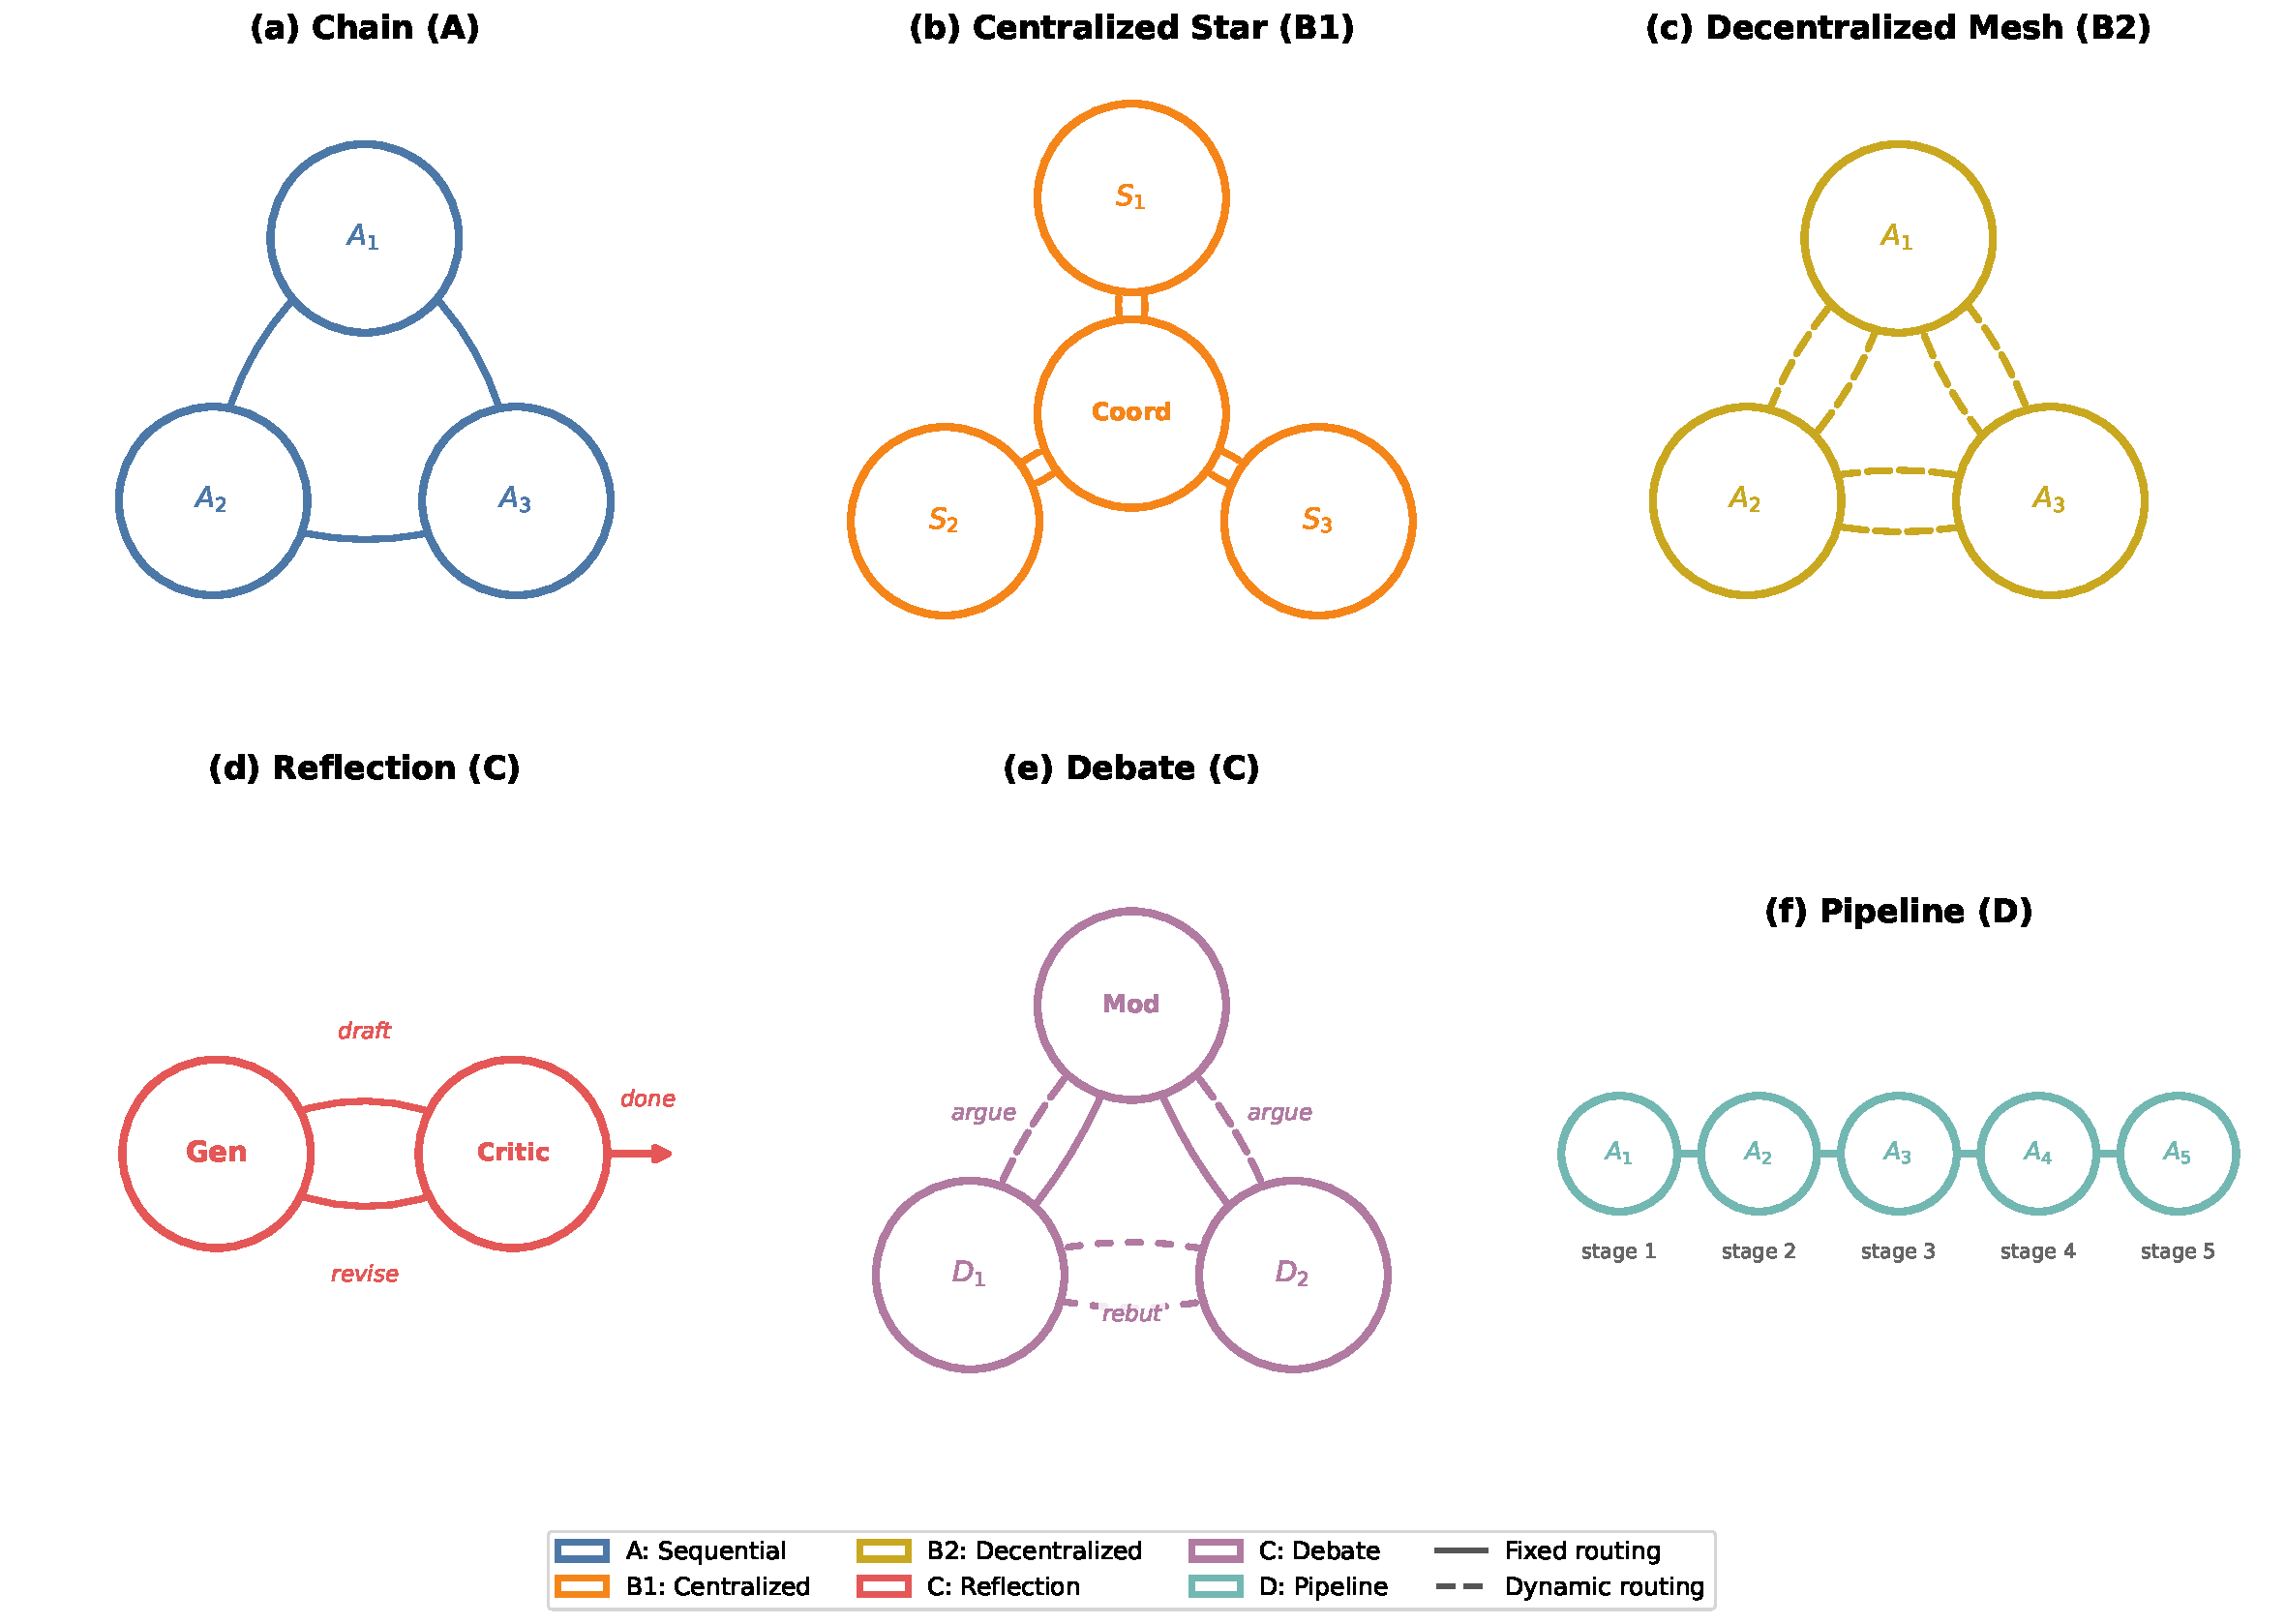
\includegraphics[width=\linewidth]{fig1_taxonomy.pdf}
    \caption{13가지 조정 패턴의 5개 범주 분류 체계. 체인(A), 스타(B1), 메시(B2), 피드백(C), 복합(D) 토폴로지.}
    \label{fig:taxonomy}
\end{figure}

\textbf{고정 순차 (범주 A) --- 체인 토폴로지.} 라운드 로빈 패턴은 고정 순서로 에이전트를 순환: $\text{Agent}_1 \to \text{Agent}_2 \to \cdots \to \text{Agent}_n \to \text{Agent}_1$. 각 에이전트는 전체 대화 이력을 보지만 라우팅에 영향을 미칠 수 없다. 이는 Masterman et al.의 체인/워터폴 토폴로지에 해당하며, MetaGPT (Hong et al., 2024)의 SOP 기반 순차 핸드오프와 동일한 구조다. 패턴: RR-2, RR-3, RR-4.

\textbf{중앙 집중형 라우팅 (범주 B1) --- 스타 토폴로지.} 전용 조정자 에이전트(Selector)가 대화 상태를 분석하여 다음 호출할 전문가를 \textbf{중앙에서 결정}한다. 이는 Masterman et al.의 스타/허브-앤-스포크 토폴로지에 해당하며, AutoGen의 SelectorGroupChat이 대표적 구현이다. 각 라우팅 결정마다 LLM 호출 오버헤드가 발생하나, 조정자가 전역 상태를 파악하여 최적 전문가를 선택할 수 있다. 패턴: Sel-3, Sel-4.

\textbf{탈중앙 핸드오프 (범주 B2) --- 메시 토폴로지.} 중앙 조정자 없이 각 에이전트가 \textbf{자율적으로 다음 에이전트에게 핸드오프}한다. 이는 Masterman et al.의 메시/스웜 토폴로지에 해당하며, OpenAI Swarm (2024)의 경량 핸드오프 루틴이 대표적이다. 에이전트 간 직접적 P2P 통신으로 조정 병목이 없으나, 턴 폭증(turn explosion)의 위험이 있다. 패턴: Swm-3, Swm-4.

\begin{quote}
\textbf{범주 B의 분리 근거.} 기존 연구에서 Selector와 Swarm을 ``동적 라우팅''으로 통합하였으나, 본 실험 결과 양자의 행동이 근본적으로 상이함을 확인하였다: Selector는 소수의 긴 모놀로그(2,100 tok/turn)를, Swarm은 다수의 짧은 핸드오프(330 tok/turn)를 생성한다. 스케일링 방향도 정반대로, Selector는 아선형($\text{sel4}/\text{sel3}=1.48\times$)이나 Swarm은 초선형($\text{swm4}/\text{swm3}=3.17\times$)이다. Tran et al. (2025)의 5-차원 협업 프레임워크에서도 \emph{구조(Structure)} 차원에서 ``중앙 집중형(centralized) vs.\ 분산형(distributed)''을 명시적으로 분리하여, 이 구분의 학술적 정당성을 지지한다.
\end{quote}

\textbf{구조화 피드백 (범주 C).} 에이전트가 명시적 피드백 루프를 통해 출력을 반복 정제한다. 반성(reflection) 패턴 (NeurIPS 2024)은 생성자와 비평가를 쌍으로 구성하고, 토론(debate) 패턴 (Du et al., ICML 2024)은 에이전트가 중재자와 함께 논거를 교환한다. 이 토폴로지는 수렴할 수 있으나 진동의 위험도 있다. 패턴: Refl-2, Refl-3, Deb-3, Deb-4.

\textbf{복합/중첩 (범주 D).} 다수의 단계 또는 계층이 파이프라인 또는 혼합 에이전트(MoA) 아키텍처로 구성된다. 파이프라인 패턴은 체인 토폴로지의 확장(체인의 체인)으로 순차 정제 단계를 통해 과제를 처리하고, MoA (ICLR 2025)는 다수의 병렬 응답을 생성 후 집약한다. 패턴: Pipe, MoA.

선행 프레임워크는 이 패턴의 부분 집합을 구현했다: AutoGen (Wu et al., 2023)은 라운드 로빈, 선택자, 스웜 패턴을 지원하고; DyTopo (Lu et al., 2026)는 라운드마다 희소 그래프를 재구성하는 동적 토폴로지 전환을 지원하며; MoA (ICLR 2025)는 계층적 집약 패턴을 도입한다. Wang et al. (2025)은 소세계 네트워크 이론을 멀티 에이전트 토론에 적용하여 원칙적 토폴로지 설계가 합의 궤적을 안정화하면서 토큰 효율성을 유지함을 보였다. MegaAgent (ACL 2025)는 대규모에서 에이전트 간 대화 토큰이 총 비용을 지배함을 보여, 토폴로지 인식 통신 효율의 필요성을 제기한다. G-Designer (Zhang et al., ICML 2025)는 변분 그래프 오토인코더로 과제 특화 통신 토폴로지를 동적 생성하여, HumanEval에서 최대 95.33\% 토큰 절감을 달성했다. AgentDropout (Wang et al., ACL 2025)은 통신 그래프 인접 행렬을 최적화하여 중복 에이전트를 동적 제거하며, 21.6\% 프롬프트 토큰 절감과 1.14점 성능 향상을 동시 달성한다. 본 연구는 이를 보완하여 \emph{종료 역학}에 집중한다---어떤 토폴로지를 선택할 것인가가 아니라, \textbf{선택된 토폴로지 내에서 팀이 언제 멈춰야 하는가}를 연구한다.

\subsection{LLM 시스템의 종료 기준}

\textbf{단일 에이전트 종료.} REFRAIN (Sun et al., 2025)은 연쇄 사고(Chain-of-Thought) 추론에서의 ``과잉 사고(overthinking)''를 이중 단계 정지 판별기와 슬라이딩 윈도우 UCB 다중 슬롯머신 제어기로 해결하여, 정확도를 유지하면서 토큰 사용량을 20--55\% 절감한다. 자기 일관성 샘플링 (Wang et al., 2023)은 다수의 추론 경로가 합의할 때 암묵적으로 수렴 감지를 사용한다.

\textbf{멀티 에이전트 종료.} Hu et al. (NeurIPS 2025)은 멀티 에이전트 토론을 위한 적응적 안정성 감지를 제안하여, 베타-이항 분포에 대한 KS 통계량으로 심판 의견이 안정화되는 시점을 감지한다 (통상 2--7라운드). Ruan \& Wang (2025)은 점진적 쿼럼 감지를 통한 조기 종료가 가능한 형식적 합의 프로토콜 Aegean을 도입하여, 답변 품질을 2.5\% 이내로 유지하면서 1.2--20배 지연 시간 절감을 달성한다. Cemri et al. (2025)은 멀티 에이전트 시스템의 3대 실패 범주 중 하나로 종료를 식별하며, 무한 루프와 조기 종료 실패를 문서화한다. SupervisorAgent (Lin et al., 2025)는 LLM 없는 컨텍스트 필터를 통한 런타임 적응적 감독으로, GAIA 벤치마크에서 성공률 저하 없이 토큰 소비를 29.45\% 절감한다.

\textbf{갭(Gap).} 포괄적인 조정 토폴로지 집합에서 종료 역학이 어떻게 변하는지를 체계적으로 연구한 선행 연구는 없다. 기존 적응적 종료는 특정 설정을 대상으로 한다: Hu et al. (2025)은 토론 패턴, Aegean은 병렬 합의, REFRAIN은 단일 에이전트 CoT. G-Designer는 토폴로지 선택을 최적화하지만 선택된 토폴로지 내에서 언제 멈출지는 연구하지 않는다. AgentDropout은 \emph{어떤 에이전트가} 참여할지를 최적화하지만 \emph{언제} 종료할지는 다루지 않는다. 본 연구는 5개 범주의 13개 패턴을 연구하고, 토폴로지 인식 적응적 종료를 제안하며, 팀이 언제 멈춰야 하는지에 대한 실증적 가이드라인을 제공함으로써 이 갭을 메운다.

\subsection{멀티 에이전트 출력의 품질 평가}

품질 지표로 G-Eval (Liu et al., 2023)을 채택하며, 평가자 LLM으로 Claude Sonnet 4.5를 사용한다. G-Eval은 인간 판단과 높은 상관이 입증된 구조화된 텍스트 품질 평가 프레임워크를 제공한다. 5개 과제 관련 차원으로 적응: 정확성(accuracy), 완전성(completeness), 일관성(coherence), 유용성(usefulness), 종합(overall), 각각 1--5 정수 척도. 오류 감지를 위해 MAST 범주와 정렬한 분류 체계를 사용한다: 환각, 사실 오류, 불완전성, 불일치, 무관성.

\begin{table}[t]
\centering
\caption{관련 연구 비교}
\label{tab:related-work}
{\small
\begin{tabular}{lcccc}
\toprule
\textbf{연구} & \textbf{패턴 수} & \textbf{토폴로지 범주} & \textbf{적응적 종료} & \textbf{수렴 감지} \\
\midrule
MAST (Cemri et al., 2025) & 2 & 토론, 투표 & 없음 & 궤적 수준 \\
REFRAIN (2025) & 1 & CoT (단일) & 있음 (판별기+UCB) & 해당 없음 \\
Hu et al. (NeurIPS 2025) & 1 & 토론 & 있음 (KS-검정) & 분포 수준 \\
Aegean (Ruan \& Wang, 2025) & 해당 없음 & 병렬 합의 & 있음 (쿼럼) & 쿼럼 수준 \\
Cemri et al. (2025) & ${\sim}5$ & 혼합 & 없음 & 사후 분석 \\
G-Designer (ICML 2025) & 동적 & GNN 생성 & 없음 (과제별 고정) & 해당 없음 \\
Scaling Agent Systems (2025) & 5 & 4개 조정 유형 & 없음 & 해당 없음 \\
Wang et al. (2025) & 1 & 토론 (소규모 세계) & 없음 & 의미 엔트로피 \\
AgentDropout (ACL 2025) & 가변 & 통신 그래프 & 없음 (에이전트 제거) & 해당 없음 \\
SupervisorAgent (2025) & 1+ & 런타임 감독 & 있음 (LLM-프리 필터) & 컨텍스트 수준 \\
\midrule
\textbf{본 연구} & \textbf{14} & \textbf{6개 범주} & \textbf{있음 (토폴로지 인식)} & \textbf{주장 수준 KS-검정} \\
 & & & & \textbf{+ 비용 예측 + 난이도 상호작용} \\
\bottomrule
\end{tabular}
}
\end{table}

%% ========================================================
\section{방법론}
%% ========================================================

\subsection{패턴 분류 체계}

고전적 MAS 토폴로지 이론 (Masterman et al., 2025)의 3대 정규 토폴로지(체인, 스타, 메시)에 피드백 루프와 복합 아키텍처를 추가하여, \textbf{5개 범주}로 조직된 13가지 조정 패턴을 연구한다 (그림~\ref{fig:taxonomy}). 각 패턴은 에이전트 수 $n$으로 매개변수화되며, 공통 종료 어휘를 공유한다 (정상 종료를 위한 TERMINATE 키워드, 안전 상한으로 \texttt{max\_messages}=25).

\begin{table}[H]
\centering
\caption{패턴 구성}
\label{tab:patterns}
{\small
\begin{tabular}{llllcll}
\toprule
\textbf{패턴} & \textbf{범주} & \textbf{토폴로지} & \textbf{에이전트} & \textbf{역할} & \textbf{라우팅} & \textbf{종료} \\
\midrule
Solo & S & 단일 & 1 & 범용 어시스턴트 & N/A & 키워드 또는 최대 \\
RR-2 & A & 체인 & 2 & 작성자, 연구자 & 고정 라운드 로빈 & 키워드 또는 최대 \\
RR-3 & A & 체인 & 3 & 작성자, 연구자, 검토자 & 고정 라운드 로빈 & 키워드 또는 최대 \\
RR-4 & A & 체인 & 4 & 작성자, 연구자, 검토자, 편집자 & 고정 라운드 로빈 & 키워드 또는 최대 \\
Sel-3 & B1 & 스타 & 3+1 & 전문가 3 + 선택자 & 중앙 LLM 라우팅 & 키워드 또는 최대 \\
Sel-4 & B1 & 스타 & 4+1 & 전문가 4 + 선택자 & 중앙 LLM 라우팅 & 키워드 또는 최대 \\
Swm-3 & B2 & 메시 & 3 & 핸드오프 전문가 3 & 자율 P2P 핸드오프 & 키워드 또는 최대 \\
Swm-4 & B2 & 메시 & 4 & 핸드오프 전문가 4 & 자율 P2P 핸드오프 & 키워드 또는 최대 \\
Refl-2 & C & 피드백 & 2 & 생성자, 비평가 & 피드백 고정 & 키워드 또는 최대 \\
Refl-3 & C & 피드백 & 3 & 생성자, 비평가, 정제자 & 피드백 고정 & 키워드 또는 최대 \\
Deb-3 & C & 피드백 & 3+1 & 토론자 3 + 중재자 & 중재 & 키워드 또는 최대 \\
Deb-4 & C & 피드백 & 4+1 & 토론자 4 + 중재자 & 중재 & 키워드 또는 최대 \\
Pipe & D & 체인의 체인 & 2+ & 단계별 팀 & 순차 단계 & 단계별 키워드 \\
MoA & D & 팬아웃/집약 & 3+ & 병렬 + 집약자 & 팬아웃/집약 & 집약자 결정 \\
\bottomrule
\end{tabular}
}
\end{table}

\subsection{과제 모음}

25개 과제를 \textbf{2차원}으로 분류한다: \emph{인지 유형} (4개)과 \emph{주제 도메인} (9개). 이 이중 분류는 ``어떤 도메인에 어떤 토폴로지가 적합한가''를 분석할 수 있게 한다 (MultiAgentBench, ACL 2025; LegalAgentBench, ACL 2025 참조). 도메인 다양성을 극대화하여 도메인별 토폴로지 적합성 분석을 가능하게 한다.

\textbf{인지 유형 (4개):}
\begin{itemize}
    \item \textbf{사실형} (7개): 지식 검색 및 종합이 필요한 질문
    \item \textbf{분석형} (9개): 구조화된 추론과 비교 분석이 필요한 문제
    \item \textbf{창의형} (6개): 창의성, 대안 사고, 설계가 필요한 개방형 과제
    \item \textbf{기술형} (3개): 전문 기술 지식과 구현이 필요한 도메인 특화 과제
\end{itemize}

\textbf{주제 도메인 (9개):}
\begin{itemize}
    \item \textbf{과학} (3개): 열역학, 광합성, 암흑물질 검출
    \item \textbf{CS} (3개): 네트워킹, LRU 캐시 구현, 아키텍처 비교
    \item \textbf{역사} (3개): 1차 대전 원인, 제국 비교, 대안 역사
    \item \textbf{철학} (3개): 칸트 vs 밀, 트롤리 문제, 정체성 사고실험
    \item \textbf{법/정치} (3개): 삼권분립, AI 저작권, 자율주행 정책
    \item \textbf{게임} (3개): 게임 설계 원리, 매치메이킹, 교육 게임
    \item \textbf{공학} (3개): 구조 하중, 수처리장, 3D 프린팅 건설
    \item \textbf{경영} (3개): AI 교육 스타트업, VC vs 부트스트래핑, EV 시장 진출
    \item \textbf{의학} (1개): mRNA vs 단백질 백신
\end{itemize}

\begin{table}[t]
\centering
\caption{과제 분포 (인지유형 $\times$ 도메인)}
\label{tab:task-distribution}
\begin{tabular}{lccccc}
\toprule
\textbf{도메인} & \textbf{사실} & \textbf{분석} & \textbf{창의} & \textbf{기술} & \textbf{합계} \\
\midrule
과학 & 1 & 1 & 1 & 0 & 3 \\
CS & 1 & 1 & 0 & 1 & 3 \\
역사 & 1 & 1 & 1 & 0 & 3 \\
철학 & 1 & 1 & 1 & 0 & 3 \\
법/정치 & 1 & 1 & 1 & 0 & 3 \\
게임 & 1 & 0 & 1 & 1 & 3 \\
공학 & 1 & 1 & 0 & 1 & 3 \\
경영 & 0 & 2 & 1 & 0 & 3 \\
의학 & 0 & 1 & 0 & 0 & 1 \\
\midrule
\textbf{합계} & \textbf{7} & \textbf{9} & \textbf{6} & \textbf{3} & \textbf{25} \\
\bottomrule
\end{tabular}
\end{table}

v1 실험에서는 각 과제를 패턴당 3회 반복 실행하여 780회 실행 ($13\text{패턴} \times 20\text{과제} \times 3\text{반복}$)을 수행했다. v2 실험에서는 대표 패턴 8개에 대해 25개 과제를 각 1회 실행하여 200회 실행 ($8\text{패턴} \times 25\text{과제}$)을 수행한다.

전체 과제 목록과 프롬프트 원문은 부록 A의 표 A1에 수록한다. 각 프롬프트는 자기 완결적이며, 사실형 과제는 평균 25단어, 창의/기술형 과제는 평균 45단어이다. 본 메인 과제 모음은 중$\sim$고 난이도이며, 실험 07에서 명시적 쉬움/보통/어려움 등급을 도입한다.

\textbf{설계 근거: 개방형 과제.} 검증 가능한 벤치마크(HumanEval, MATH, MMLU 등)가 아닌 개방형 생성 과제를 \textbf{의도적으로} 선택했다. 종료 역학 연구에는 \textbf{턴에 걸쳐 품질이 연속적으로 변화}하는 과제가 필요하기 때문이다. 검증 가능한 벤치마크는 이진 결과(통과/실패)를 생성하여 턴별 품질 궤적, 수렴 패턴, 한계 효용 분석이 의존하는 점진적 품질 포화를 드러낼 수 없다. 개방형 과제는 최적 종료 시점 식별, 종료 후회 측정, 토폴로지 간 수렴 속도 비교에 필요한 풍부한 품질 곡선을 생성한다. 이 설계 선택은 관련 멀티 에이전트 평가 연구와 일치한다: MAST (Cemri et al., 2025)는 궤적 수준 품질 연구에, Hu et al. (2025)는 수렴 연구에 개방형 과제를 사용한다. 코드 생성이나 수학적 추론에서의 종료 역학은 다를 수 있으며 (5.3절), 이러한 과제로의 확장은 중요한 향후 방향이다.

\subsubsection{에이전트 시스템 프롬프트}

각 에이전트는 전문성과 행동 기대치를 정의하는 역할별 시스템 프롬프트를 받는다. 모든 프롬프트는 공통 구조를 공유한다: (1) 역할 정의, (2) 응답 가이드라인, (3) 종료 지시 (``과제가 완료되면 TERMINATE라고 말하세요'').

\textbf{범주 A (라운드 로빈):} 에이전트에 상호 보완적 역할---Writer(초안 생성), Researcher(사실 보강), Reviewer(완전성 평가), Editor(문체 정제)---을 부여한다. 각 에이전트는 처음부터 다시 쓰지 않고 선행 기여에 기반하도록 지시받는다.

\textbf{범주 B1 (셀렉터):} 셀렉터 에이전트는 라우팅 프롬프트를 받는다: ``대화를 분석하고 다음 턴에 가장 적합한 전문가를 선택하세요.'' 전문가 에이전트는 범주 A와 동일한 역할 프롬프트를 받는다.

\textbf{범주 B2 (스웜):} 각 에이전트는 핸드오프 도구(\texttt{transfer\_to\_<agent>})를 받으며, ``당신의 부분을 완료한 후 다음 단계에 적합한 에이전트에게 넘기세요. 과제가 완전히 해결되면 TERMINATE라고 말하세요''라는 지시를 받는다.

\textbf{범주 C (피드백):} 반성 패턴은 Generator(``포괄적 응답 생성'')와 Critic(``정확성, 완전성, 일관성 평가; 구체적 피드백 제공 또는 만족스러우면 APPROVED'')을 사용한다. 토론 패턴은 Debater(``주제에 대한 가장 강력한 논거 제시'')와 Moderator(``논거 종합 후 합의 또는 입장이 명확해지면 VERDICT 발행'')를 사용한다.

\textbf{범주 D (복합):} 파이프라인은 순차 전문가를, MoA는 병렬 생성자와 Aggregator(``모든 응답의 최선 요소를 통합 답변으로 결합'')를 사용한다.

14개 패턴의 전체 시스템 프롬프트는 보충 코드 저장소에서 제공한다.

\subsection{실험 프레임워크}

모든 실험은 Claude Haiku 4.5를 기반 모델로 래핑한 커스텀 \texttt{ClaudeCLIChatCompletionClient}와 함께 AutoGen 프레임워크를 사용한다. 이는 SDK의 \texttt{models\_usage} 추적을 통해 호출별 토큰 수를 캡처하면서 모든 패턴에서 일관된 LLM 행동을 제공한다. 교차 모델 검증으로 GPT-4o-mini를 사용하여 발견의 일반화 가능성을 평가한다(4.6절).

\textbf{실행별 캡처 지표:}
\begin{itemize}
    \item \emph{지속 시간}: \texttt{team.run()} 시작부터 완료까지의 벽시계 시간
    \item \emph{턴 수}: 대화의 총 메시지 수
    \item \emph{에이전트 턴 수}: 비시스템 에이전트의 메시지 수
    \item \emph{토큰 사용량}: LLM 호출별 프롬프트 토큰(입력)과 완성 토큰(출력)
    \item \emph{종료 사유}: 팀 종료 방식 (키워드, \texttt{max\_messages}, 오류)
    \item \emph{품질 점수}: G-Eval 평가 (실험 02만)
    \item \emph{수렴 지점}: KS-검정 안정성 (실험 03만)
\end{itemize}

\subsection{7개 실험}

\textbf{실험 01: 패턴 효율성} (780회). 전체 과제 모음에서 13개 패턴의 지속 시간, 턴 수, 에이전트 턴, 토큰 사용량을 비교한다. Kruskal--Wallis 검정으로 토폴로지 범주가 효율의 유의한 예측 변수인지 검증한다.

\textbf{실험 02: 종료 품질} (100회). 5개 대표 패턴(범주당 하나)에 대해 20개 과제에서 각 에이전트 턴에 G-Eval 스코어링을 적용하여 품질 궤적을 구축한다 (100회 실행, 276개 턴별 품질 점수). 종료 후회(실제와 최적 종료 시점의 차이)를 식별한다.

\textbf{실험 03: 수렴 감지} (분석만). 실험 01의 메시지 데이터로 KS-검정 수렴 지표를 산출하여, 범주 간 수렴 속도를 비교한다. 피드백 패턴이 순차 패턴보다 빠르게 수렴하는지 검증한다.

\textbf{실험 04: 오류 귀인} (분석만). 실험 01과 02의 오류를 8개 유형으로 분류하고, 토폴로지 특성과의 오류 분포 상관을 분석한다. 패턴별 오류 시그니처를 검증한다.

\textbf{실험 05: 적응적 종료} (800회). 적응적 $\Delta U$ 기반 종료와 키워드 베이스라인을 비교하는 통제 실험. 8개 대표 패턴 전체에서 25개 과제를 3개 $\lambda$값(0.0, 0.1, 0.5)으로 실행하여 200회 베이스라인 + 600회 적응적 = 800회 실행. $\Delta U(t) = \Delta Q(t) - \lambda \cdot \Delta C(t) \to 0$이 실용적 종료 신호로 기능하는지 평가한다.

\textbf{실험 06: 토폴로지 특성 기반 비용 예측} (분석만). 실험 01 데이터(718회)로 4개 회귀 모델(선형, Ridge, Lasso, Random Forest)을 학습하여, 사전 실행 토폴로지 특성(패턴 범주, 에이전트 수, 최대 메시지 수, 과제 범주, 상호작용 항 \texttt{agent\_count $\times$ max\_messages})으로 런타임 비용(토큰, 턴 수, 지속 시간)을 예측한다. 5-fold 교차 검증과 실험 05 베이스라인 데이터(200회)에 대한 홀드아웃 예측으로 평가한다.

\textbf{실험 07: 과제 난이도 상호작용} (225회). 5개 대표 패턴(solo, swm3, sel3, refl2, debate3---범주당 하나)과 15개 난이도 등급 과제(5개 도메인 $\times$ 3개 난이도: 쉬움, 보통, 어려움)를 3회 반복으로 교차한다. Kruskal--Wallis 검정으로 주효과 및 상호작용을 검증하고, G-Eval 채점으로 난이도 인식 추천 매트릭스를 도출한다.
